\providecommand{\main}{../..}
\documentclass[\main/notes.tex]{subfiles}

\begin{document}
	\setcounter{chapter}{10}
	\chapter{Systems Analysis}
		\section{An Overview of Systems Development}
			\begin{definition}{The Development Team}
				A team that consists of users, managers, systems development specialists, various support personnel and other stakeholders.

				Responsible for determining the objectives of the new information system, and delivering a system that meets these objectives.

				\begin{description}
					\item[Project] A planned collection of activities that achieves a goal, such as constructing a new manufacturing plant, or developing a new decision support system. Should have as defined starting and ending point.
					\item[Project Manager] A manager that is responsible for coordinating all people and resources needed to complete the project on time. Can be an IS person inside the organisation, or an external consultant. They need technical, business, and people skills. Usually responsible for controlling project quality, training personnel, facilitating communication, managing risks, and acquiring any necessary equipment.
					\item[Stakeholders] People who, either themselves or through the area of the organisation they represent, ultimately benefit from the systems development project.
					\item[Users] People who will interact with the system regularly. Can be employees, managers, or suppliers.
					\item[Systems Analyst] A professional who specialises in analysing and designing business systems.
						\begin{description}
							\item[Specialist Business Analysts] Experts in the business who try to identify ways in which new information systems can improve the current business processes.
						\end{description}
					\item[Programmer] Responsible for modifying or developing programs to satisfy user requirements. A programmer  takes plans from the systems analyst, and builds or modifies the necessary software.
					\item[Team Leader] Responsible for the development team. Can be from the IS department, a manager from the company, or a consultant. Needs both technical and people skills.
				\end{description}
			\end{definition}
			\subsection[Information Systems Planning]{Information Systems Planning and Aligning Organisation and IS Goals}
				\begin{definition}{Information Systems Planning}
					Translating strategic and organisational goals into systems development initiatives.

					Strategic goals must be finite, measurable, and tangible.
				\end{definition}
				\begin{sidenote}{The Steps of IS Planning}
					\begin{center}
						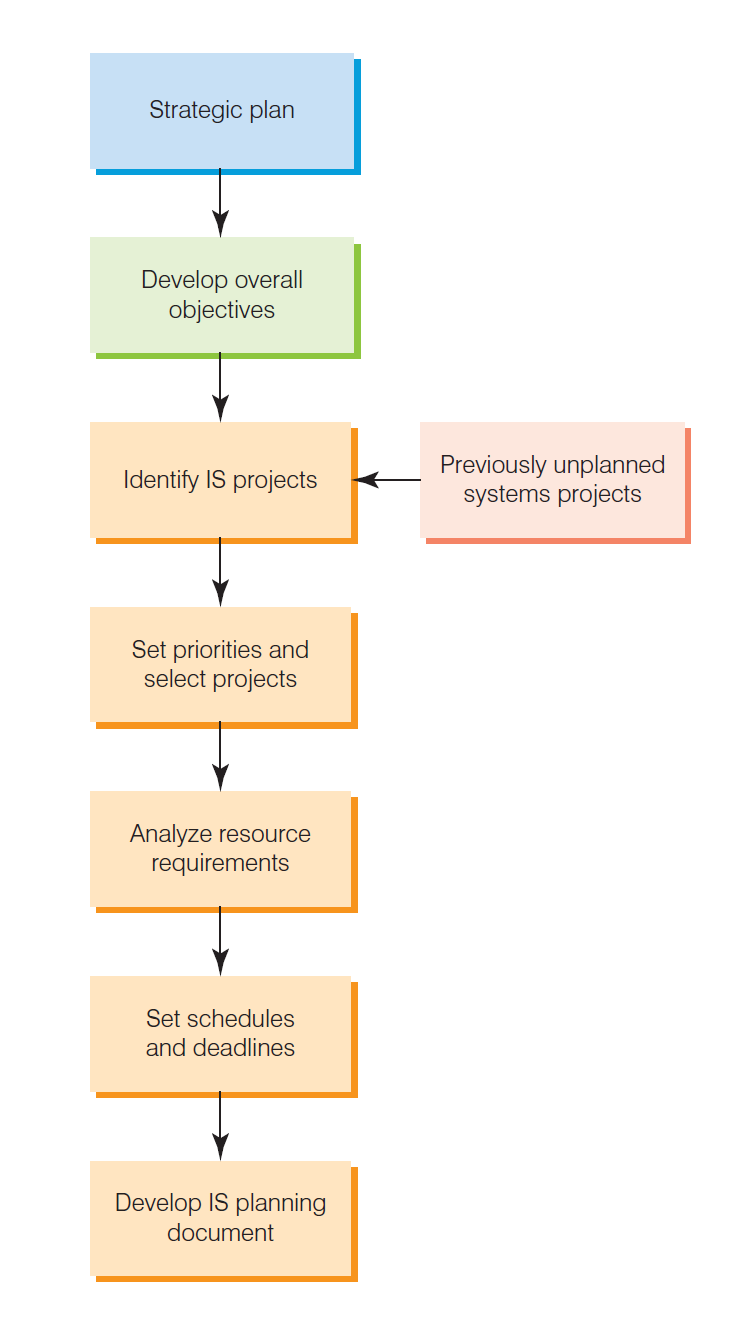
\includegraphics[width=0.6\textwidth]{chapter11/is_planning_steps.png}
					\end{center}
				\end{sidenote}
				\pagebreak
				\begin{definition}{Creative Analysis}
					The investigation of new approaches to existing problems. 

					Typically, inspired by people and events not directly related to the problem.
				\end{definition}
				\begin{definition}{Critical Analysis}
					The unbiased and careful questioning of whether system elements are related in the most effective ways.
					\begin{itemize}[nosep]
						\item Question statements and assumptions.
						\item Identify and resolve objectives and orientations that conflict.
					\end{itemize}
				\end{definition}
			\subsection{Establishing Objectives for Systems Development}
				\begin{sidenote}{Overall Objective}
					The overall objective of systems development is to achieve business goals, not technical goals, by delivering the right information to the right person at the right time.
				\end{sidenote}
				\begin{definition}{Critical Success Factors (CSFs)}
					Factors that are essential to the success of certain function areas of an organisation.
				\end{definition}
				\begin{definition}{Performance Objectives}
					The extent to which a system performs as desired.
					\begin{multicols}{2}
						\begin{itemize}[nosep]
							\item The quality or usefulness of the output
							\item The accuracy of the output
							\item The quality or usefulness of the format of the output
							\item The speed at which output is generated
							\item The scalability of the resulting system
							\item The degree to which business risk is reduced
						\end{itemize}
					\end{multicols}
				\end{definition}
				\begin{definition}{Cost Objectives}
					The costs associated with the system, should be minimised.
					\begin{multicols}{2}
						\begin{itemize}[nosep]
							\item Development costs
							\item Costs related to the uniqueness of the system application
							\item Fixed investments in hardware and related equipment
							\item Ongoing operating costs of the system
						\end{itemize}
					\end{multicols}
				\end{definition}
				Performance objectives and cost objectives should be balanced.

	\vbox{\rulechapterend}
\end{document}